%\author[Clemens A. Schächter]{Nix}


\beamertemplatenavigationsymbolsempty{}

\logo{
\includegraphics[height=1cm]{Bilder/logo}}

\section{Experiments}   
%\subsection{Simple simulated dataset}
%\begin{frame}
%\frametitle{Experiments: Simple simulated dataset}
%begin{itemize}
%	\item[] $\mathrm{D}=\{(\mathbf{x}_i,\mathbf{y}_i)\}_{i=1}^{2500}$
%	\item[] $\mathbf{x}_i\sim\mathcal{N}(0,1), \mathbf{y}_i= \mathbf{x}_i^2+\frac{1}{8}\mathbf{z}_i, \mathbf{z}_i\sim\mathcal{N}(0,1)$
%	\item[] Architecture $(1,30,30,1)$
%	\item[]MSE
%\end{itemize}
%\begin{figure}[h]      
%	\centering      
%	\hspace*{-0.6cm}
%	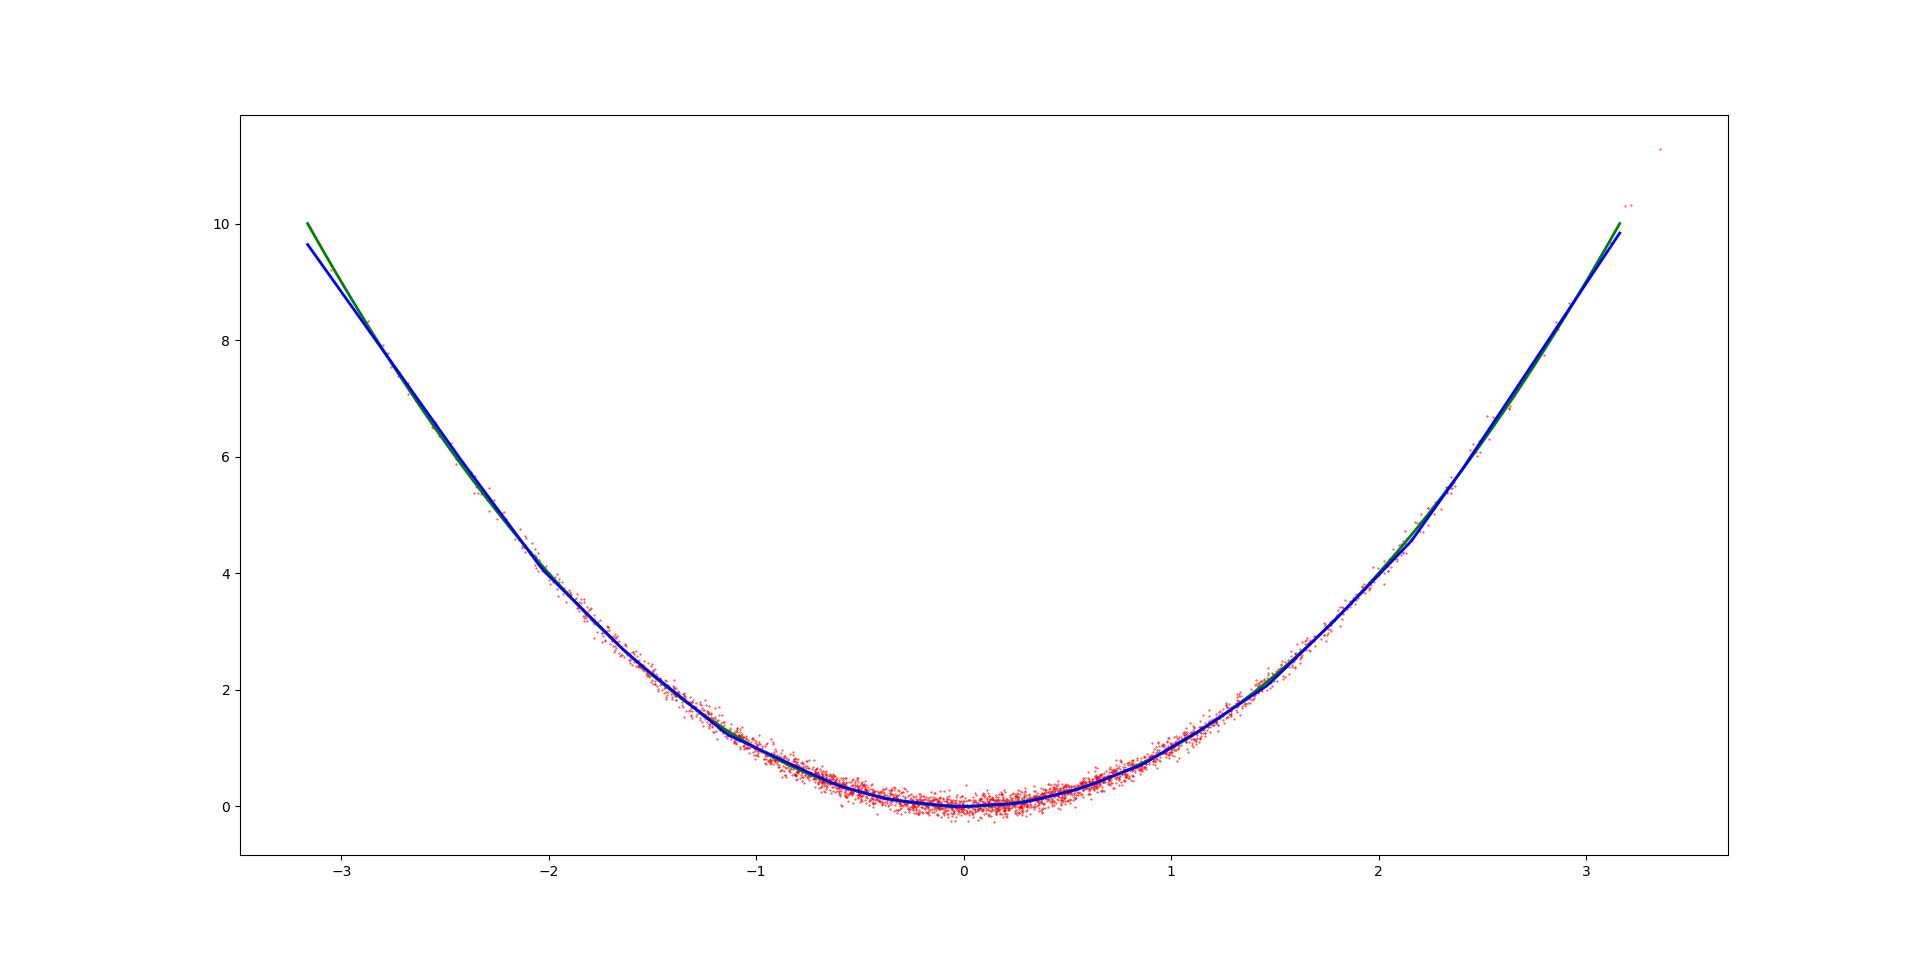
\includegraphics[scale=0.25, trim={0, 0, 0, 0}]{Bilder/Toy_Data}    
 %\end{figure}
%\end{frame}

%\begin{frame}
%\frametitle{Experiments: Simple simulated dataset}
%\begin{figure}[h]      
%	\centering      
%	\hspace*{-0.6cm}
%	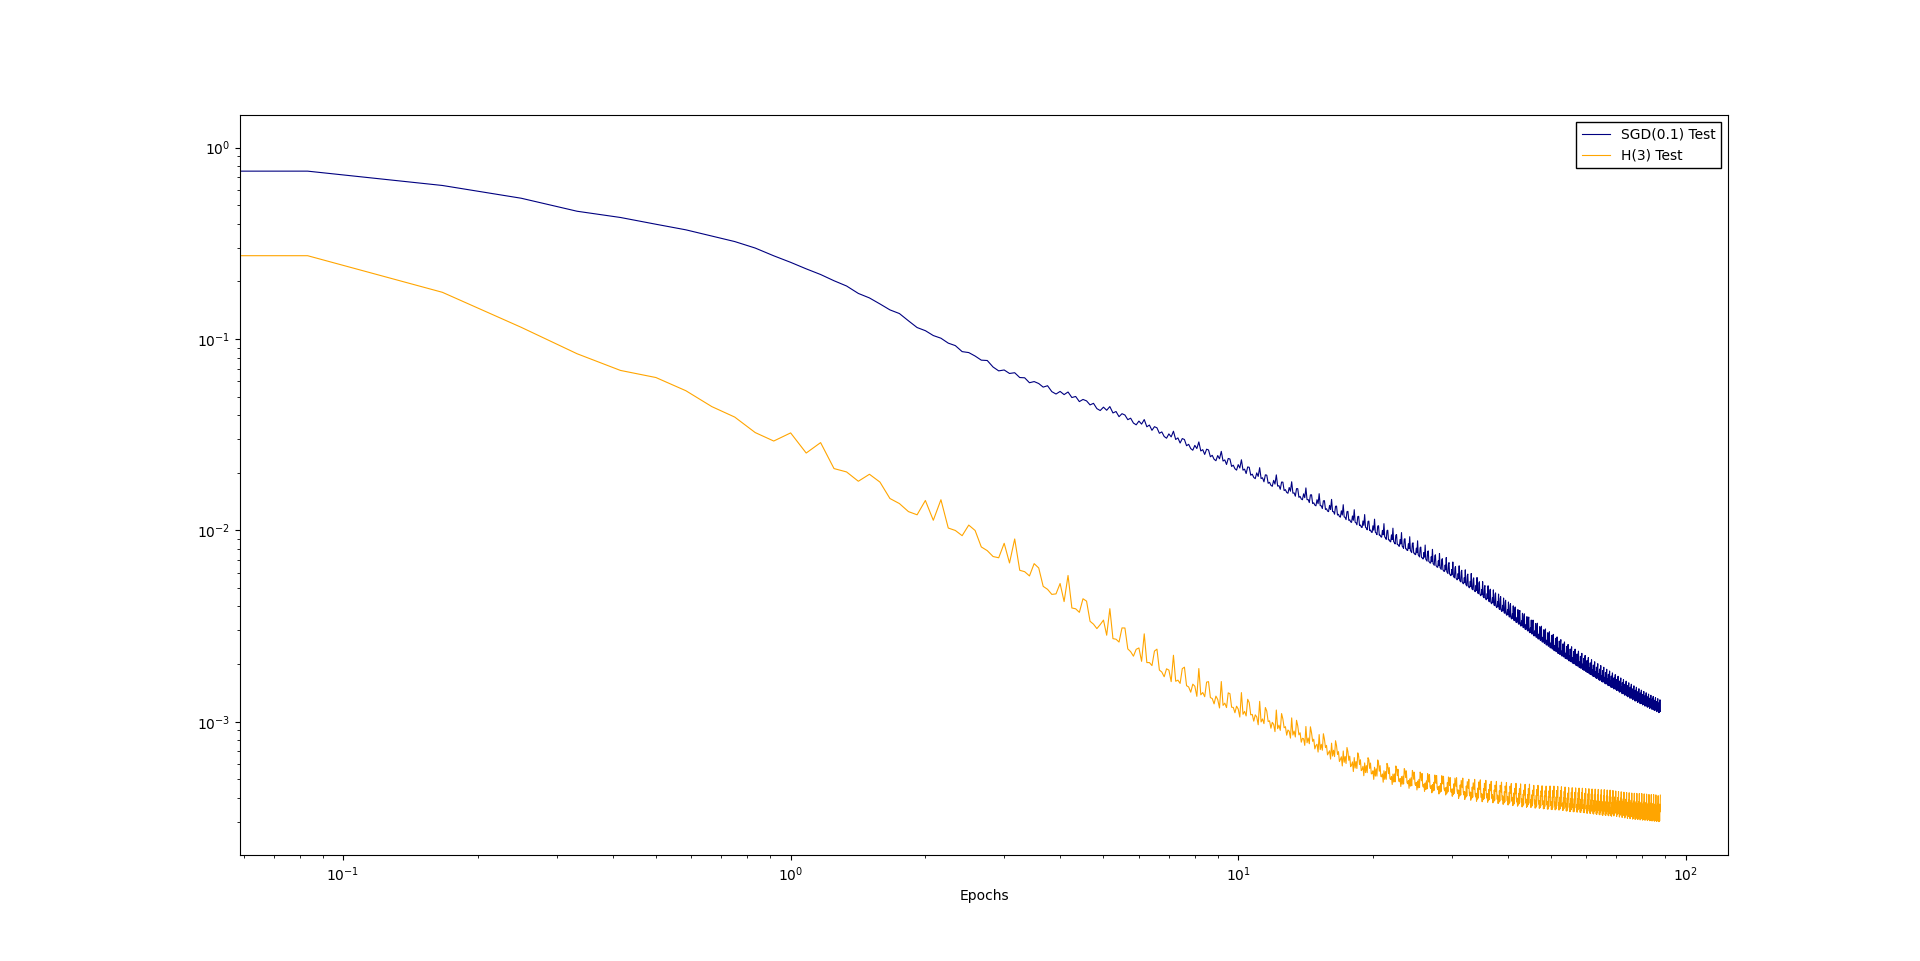
\includegraphics[scale=0.26, trim={50, 0, 0, 50}]{Bilder/Figure_3}    
%\end{figure}
%\end{frame}

%\begin{frame}
%\frametitle{Experiments: Simple simulated dataset}
%\begin{figure}[h]      
%	\centering      
%	\hspace*{-0.6cm}
%	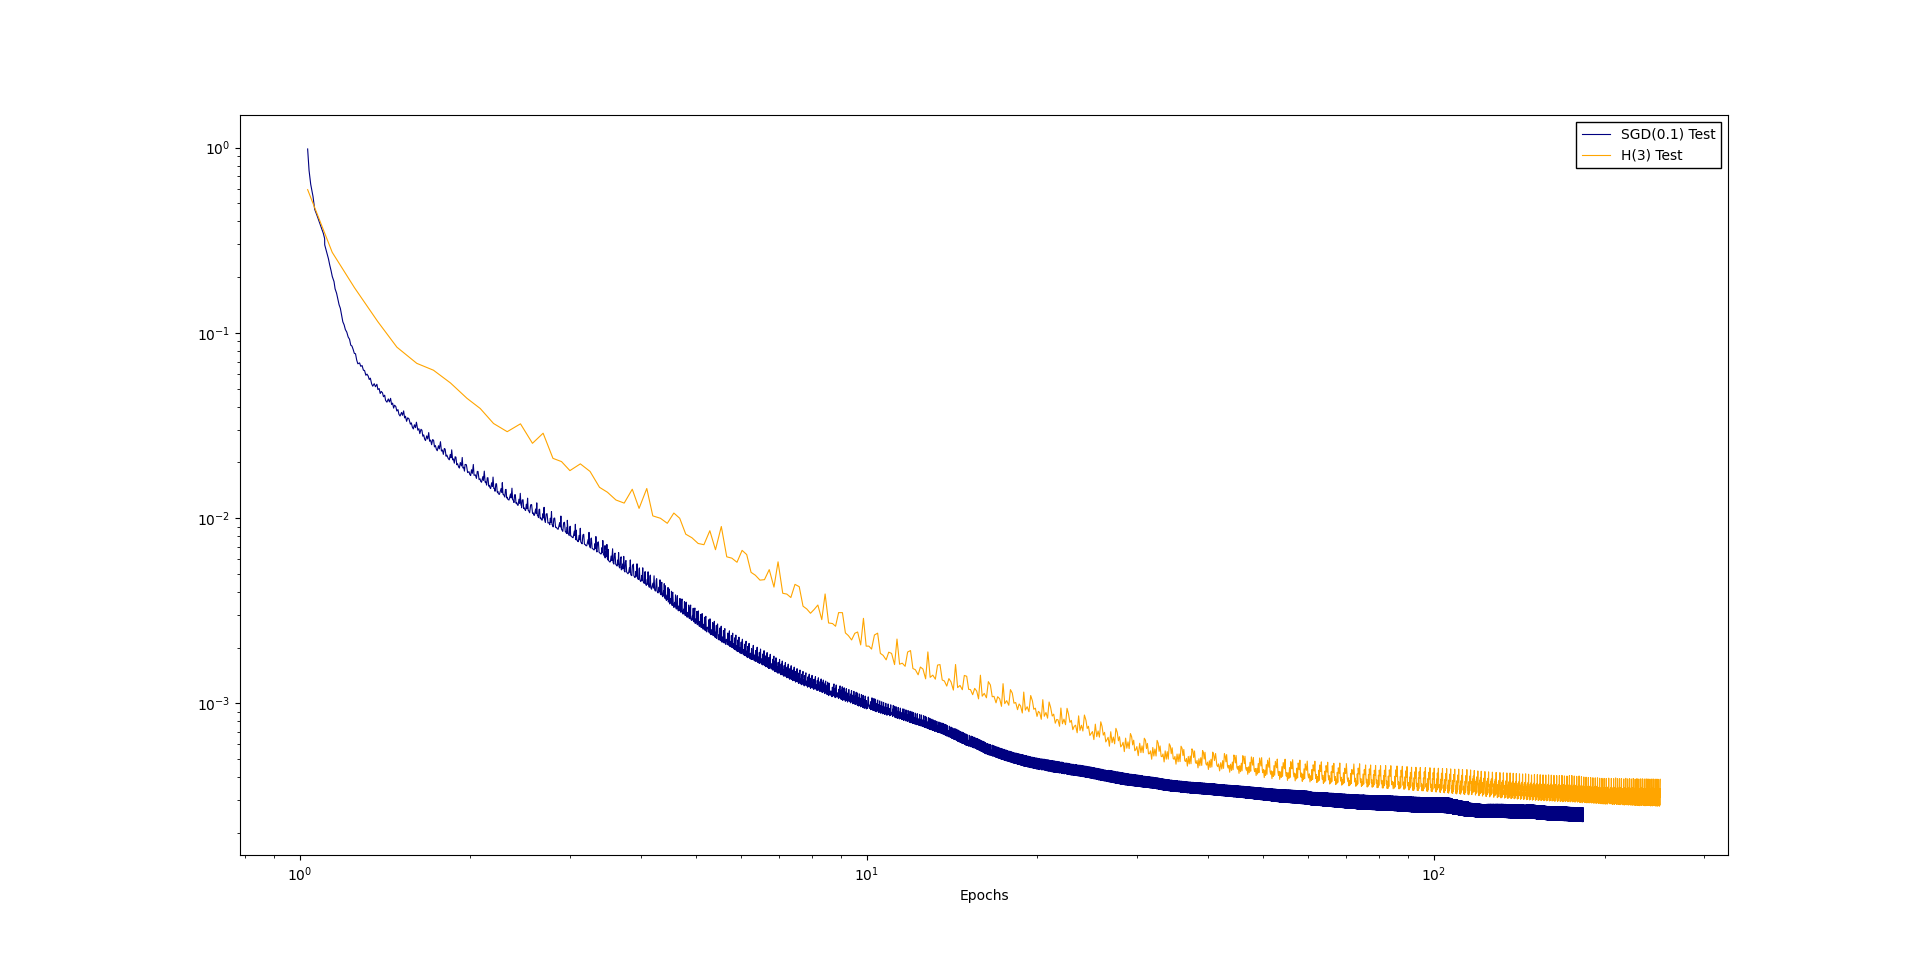
\includegraphics[scale=0.26, trim={50, 0, 0, 50}]{Bilder/Figure_2}    
%\end{figure}
%\end{frame}


\subsection{MNIST}
\begin{frame}
\frametitle{Experiments: MNIST dataset}
\begin{itemize}
\item[] Code implemented with Tensorflow
\item[] Handwritten digits from $0,\ldots,9$
\item[] 60.000 Train Images, 10.000 Test Images 
\item[] Architecture $(784,500,10)$
\item[] Benchmark to Beat: 1.6\% Error Rate
\item[] Softmax with Crossentropy-loss
\end{itemize}
\begin{figure}[h]      
	\centering      
	\hspace*{-0.6cm}
	\includegraphics[scale=0.4, trim={40, 0, 0, 0}]{Bilder/MNIST_Data}    
\end{figure}
%Bild 4 Mnist Data
%Bild 5 Results
\end{frame}

\begin{frame}
\frametitle{Experiments: MNIST dataset}
\begin{figure}[h]      
	\centering      
	\hspace*{-0.6cm}
	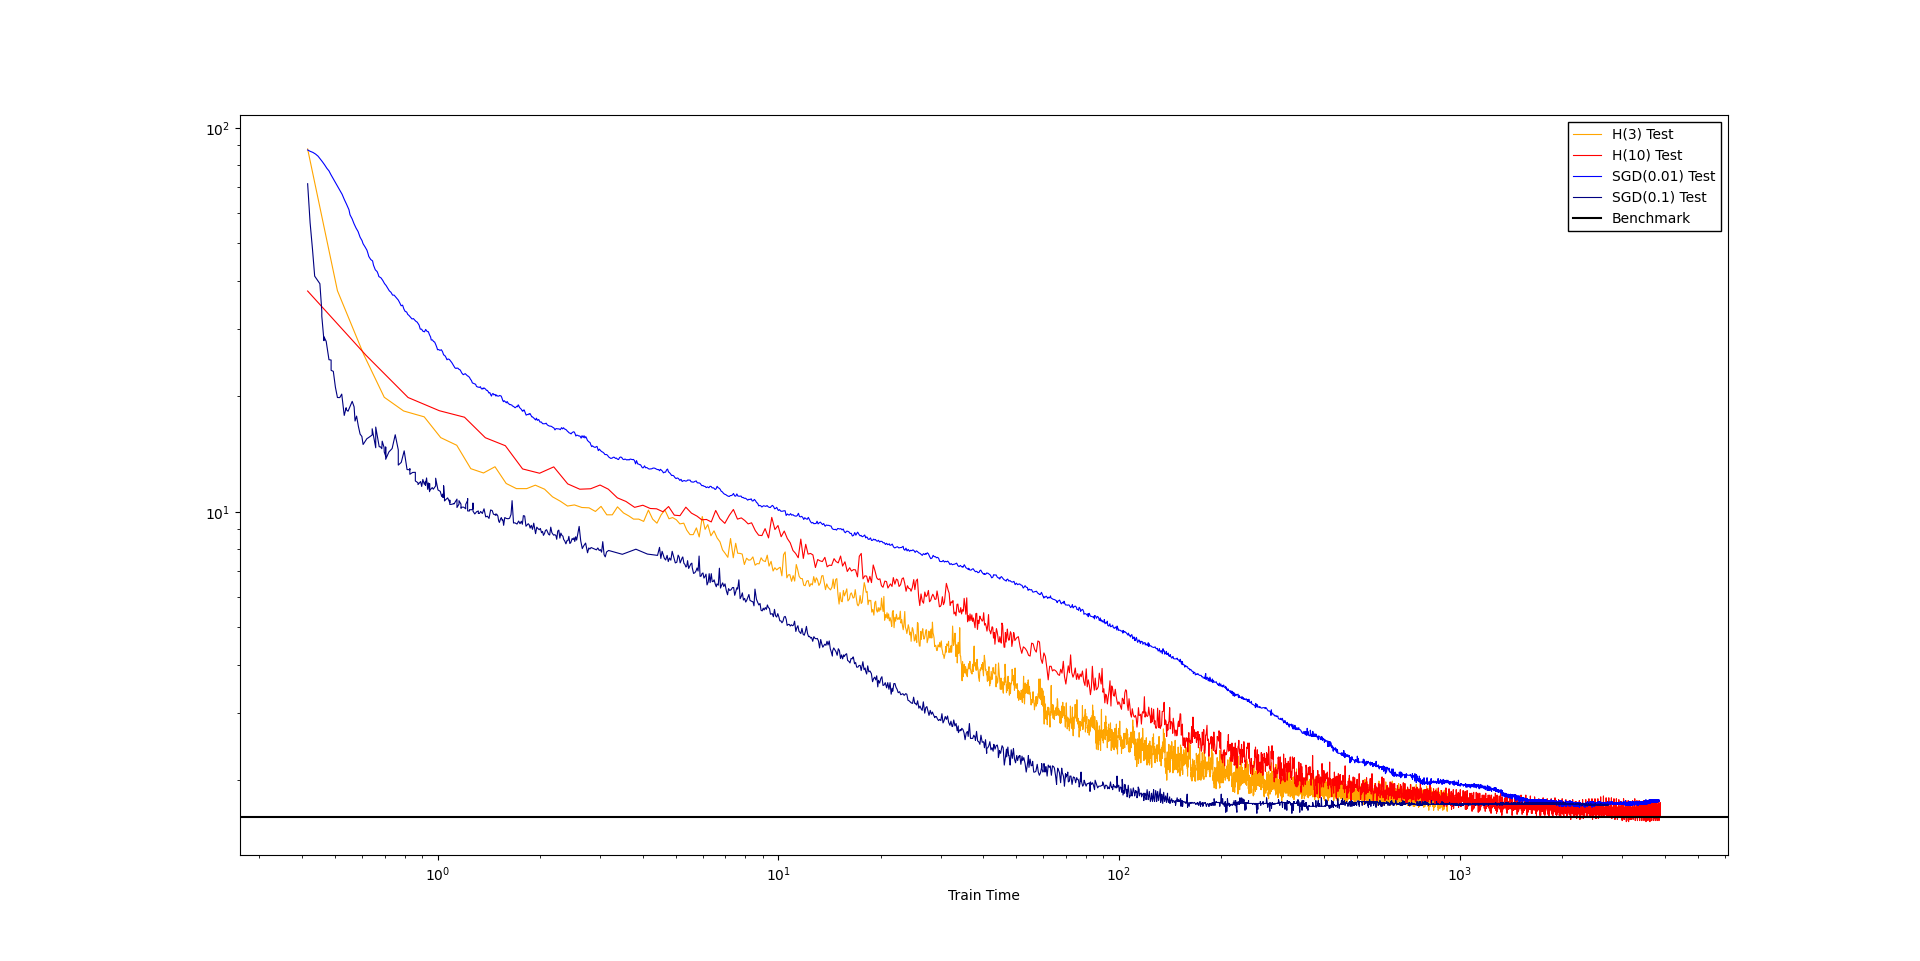
\includegraphics[scale=0.26, trim={50, 0, 0, 50}]{Bilder/Figure_1}    
\end{figure}
\end{frame}


%\author[Clemens A. Schächter]{Nix}


%\beamertemplatenavigationsymbolsempty{}

%\logo{
\includegraphics[height=1cm]{Bilder/logo}}

%\section{Experiments}   
%\subsection{Simple simulated dataset}
%\begin{frame}
%\frametitle{Experiments: Simple simulated dataset}
%\begin{itemize}
%	\item[] 
%\end{itemize}
%\end{frame}
%\subsection{MNIST}
%\begin{frame}
%\frametitle{Experiments: MNIST dataset}
%\begin{itemize}
%	\item[] 
%\end{itemize}
%\end{frame}




%\begin{frame}
%\frametitle{SDE Beispiele}
%\begin{tiny}SDE-Pfad-Simulationen von Ben Deitmar\end{tiny}
%\begin{figure}[h!]
%\begin{minipage}{0.4\textwidth}
%		%\begin{mdframed}[style=innersmall]
%		\center{}
%		\includegraphics[scale=0.27]{Bilder/SDE_sig=0}
%		\begin{tiny} $\mathrm{d}X_{t}=X_{t}\text{ }\mathrm{d}t+0\text{ }\mathrm{d}W_{t},$ $X_{0}=1$\\ $\mathrm{d}X_{t}=X_{t}\text{ }\mathrm{d}t+0\text{ }\circ \mathrm{d}W_{t},$ $X_{0}=1$ \end{tiny}
%		\center{}
%		\includegraphics[scale=0.27]{Bilder/SDE_BB}
%		\begin{tiny} $\mathrm{d}X_{t}=0\mathrm{d}t+\mathrm{d}W_{t},$ $X_{0}=1$\\ $\mathrm{d}X_{t}=0\mathrm{d}t+\circ\mathrm{d}W_{t},$ $X_{0}=1$\end{tiny}
%\center{}
%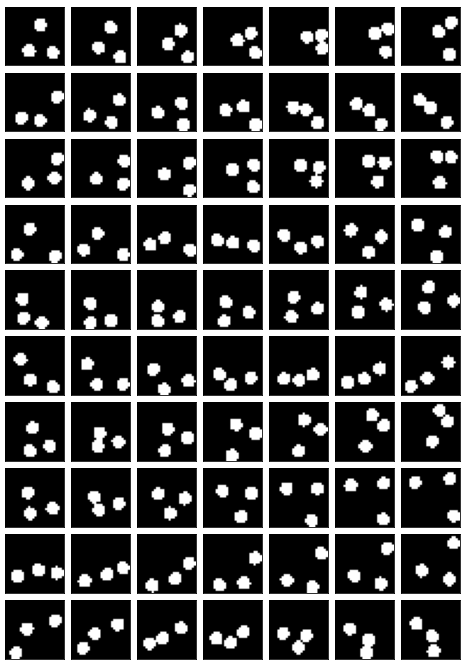
\includegraphics[scale=0.15]{Bilder/bouncingBalls_ODEorig2}
%\end{mdframed}
%	\end{minipage}
%\begin{minipage}{0.4\textwidth}
%\begin{mdframed}[style=innersmall]
%		\center{}
%		\includegraphics[scale=0.27]{Bilder/SDE_mu=x_sig=tt}
%		\begin{tiny} $dX_{t}=X_{t}\text{ }\mathrm{d}t+t^{2}\text{ }\mathrm{d}W_{t},$ $X_{0}=1$\\
%		$dX_{t}=X_{t}\text{ }\mathrm{d}t+t^{2}\text{ }\circ\mathrm{d}W_{t},$ $X_{0}=1$\end{tiny}
%\center{}
%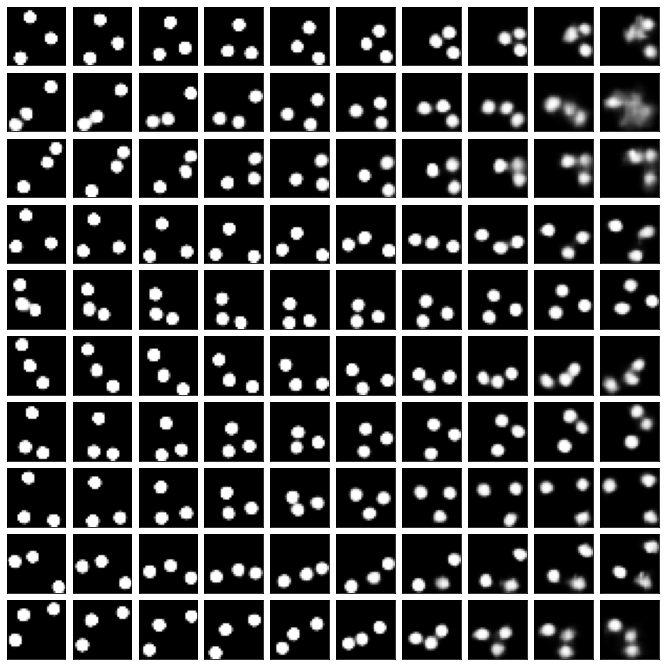
\includegraphics[scale=0.15]{Bilder/bouncingBalls_ODE}
%\end{mdframed}
%\end{minipage}
%\begin{minipage}{0.2\textwidth}
%\begin{mdframed}[style=innersmall]
%\center{}
%\includegraphics[scale=0.27]{Bilder/SDE_mu=x_sig=tt_x0=0}
%\begin{tiny} $dX_{t}=0+X_{t}\text{ }\mathrm{d}t+t^{2}\text{ }\mathrm{d}W_{t},$ $X_{0}=0$\\ $dX_{t}=0+X_{t}\text{ }\mathrm{d}t+t^{2}\text{ }\circ\mathrm{d}W_{t},$ $X_{0}=0$\end{tiny}
%\center{}
%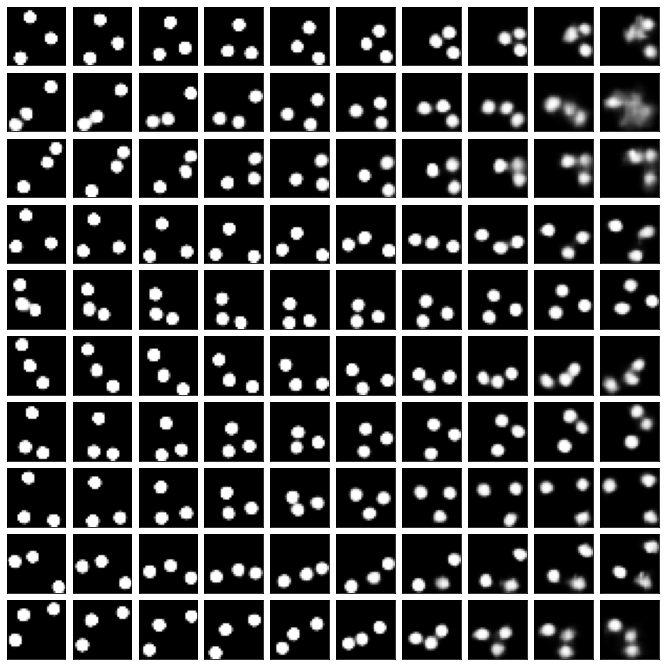
\includegraphics[scale=0.15]{Bilder/bouncingBalls_ODE}
%\end{mdframed}
% \end{minipage}
% \end{figure}
%\end{frame}
